%\documentclass{recpad2k}
\documentclass[extendedabs]{recpad2k}

%% Enter your paper number here for the review copy
\recpadreviewcopy{??}

\title{Clustering DNA sequences by relative compression}

% Enter the paper's authors in order
\addauthor{Morteza Hosseini}{seyedmorteza@ua.pt}{1}
\addauthor{Diogo Pratas}{pratas@ua.pt}{1}
\addauthor{Armando J. Pinho}{ap@ua.pt}{1}

% Enter the institutions
\addinstitution{
 IEETA/DETI,\\
 University of Aveiro
}

\runninghead{Student, Prof, Collaborator}{RECPAD Author Guidelines}

% Any macro definitions you would like to include
% These are not defined in the style file, because they don't begin
% with \bmva, so they might conflict with the user's own macros.
% The \bmvaOneDot macro adds a full stop unless there is one in the
% text already.
\def\eg{\emph{e.g}\bmvaOneDot}
\def\Eg{\emph{E.g}\bmvaOneDot}
\def\etal{\emph{et al}\bmvaOneDot}

%------------------------------------------------------------------------- 
% Document starts here
\begin{document}

\maketitle

\begin{abstract}
   This document demonstrates the format requirements for papers submitted
   to the Portuguese Conference on Pattern Recognition.  The format is designed for
   easy on-screen reading, and to print well at one or two pages per sheet.
   Additional features include: pop-up annotations for
   citations~\cite{Authors06,Mermin89}; a margin ruler for reviewing; and a
   greatly simplified way of entering multiple authors and institutions.
\end{abstract}

%------------------------------------------------------------------------- 
\section{Introduction}


%------------------------------------------------------------------------- 
\section{Results}
The proposed method is implemented and publicly available at \url{github.com/smortezah/Clusico}, under GPLv3 license. The machine used for the tests had an 8-core 3.40 GHz Intel\textsuperscript{\scriptsize\textregistered} Core{\scriptsize\texttrademark} i7-6700 CPU with 32~GB RAM.

For the experiments, we have used 30 mitochondrial DNA (mtDNA) sequences from three groups of Actinopterygii (Ray-finned fishes), Chondrichthyes (Cartilaginous fishes) and Mammalia, that can be downloaded from \url{www.ncbi.nlm.nih.gov/nuccore}. Each groups contains 10 sequences and their sizes varies from 16,189 to 18,431 bases.

In order to classify the sequences, we first ran GeCo~\cite{pratas2016efficient} on all sequences, considering them as references as well as targets, to find similarity of sequences to each other. For measuring the similarity, normalized relative compression (NRC) were used, that can be calculated as~\cite{pratas2018comparison}
\begin{equation}
   \mathrm{NRC} (x||y) = \frac{C (x||y)}{|x|\, \log_2 |\Phi|},
\end{equation}
in which $C (x||y)$ is the information in the sequence $x$ and is obtained by compressing $x$ relatively to the sequence $y$, $|x|$ is the size of sequence $x$ and $|\Phi|$ is the cardinality of input DNA sequences, i.e. $ \mathrm{size}(\{A, C, G, T\}) = 4 $. Values of NRC falls within the range $(0, 1]$ and the more similar two sequences are, the less is this value.

In the next step, we used weighted pair group method with arithmetic mean (WPGMA), which is a bottom-up hierarchical clustring method, to classify the sequences based on NRC values. The WPGMA algorithm employs a similarity matrix to construct a rooted tree (dendrogram)~\cite{sokal58a, clifford2011comparison}.

Figure~\ref{fig.nrc}a shows similarity of different sequences (NRC values), obtained by GeCo. As is show, when a sequence is compressed relatively to itself, the NRC value will be approximately 0. These cases are shown with red squares.

Figure~\ref{fig.nrc}b demonstrates the result of classification of the sequences, which is obtained by WPGMA algorithm. The sequences in Mammalia, Chondrichthyes and Actinopterygii groups are shown with red, green and blue colors, respectively. On top of this figure, the dendrogram is plotted, which shows similarity of different sequences within each group and also, similarity of different groups. As it is show, the two groups of Chondrichthyes and Actinopterygii, that are fishes, are more similar to each other, in comparison with Mammalia.

\begin{figure*}
   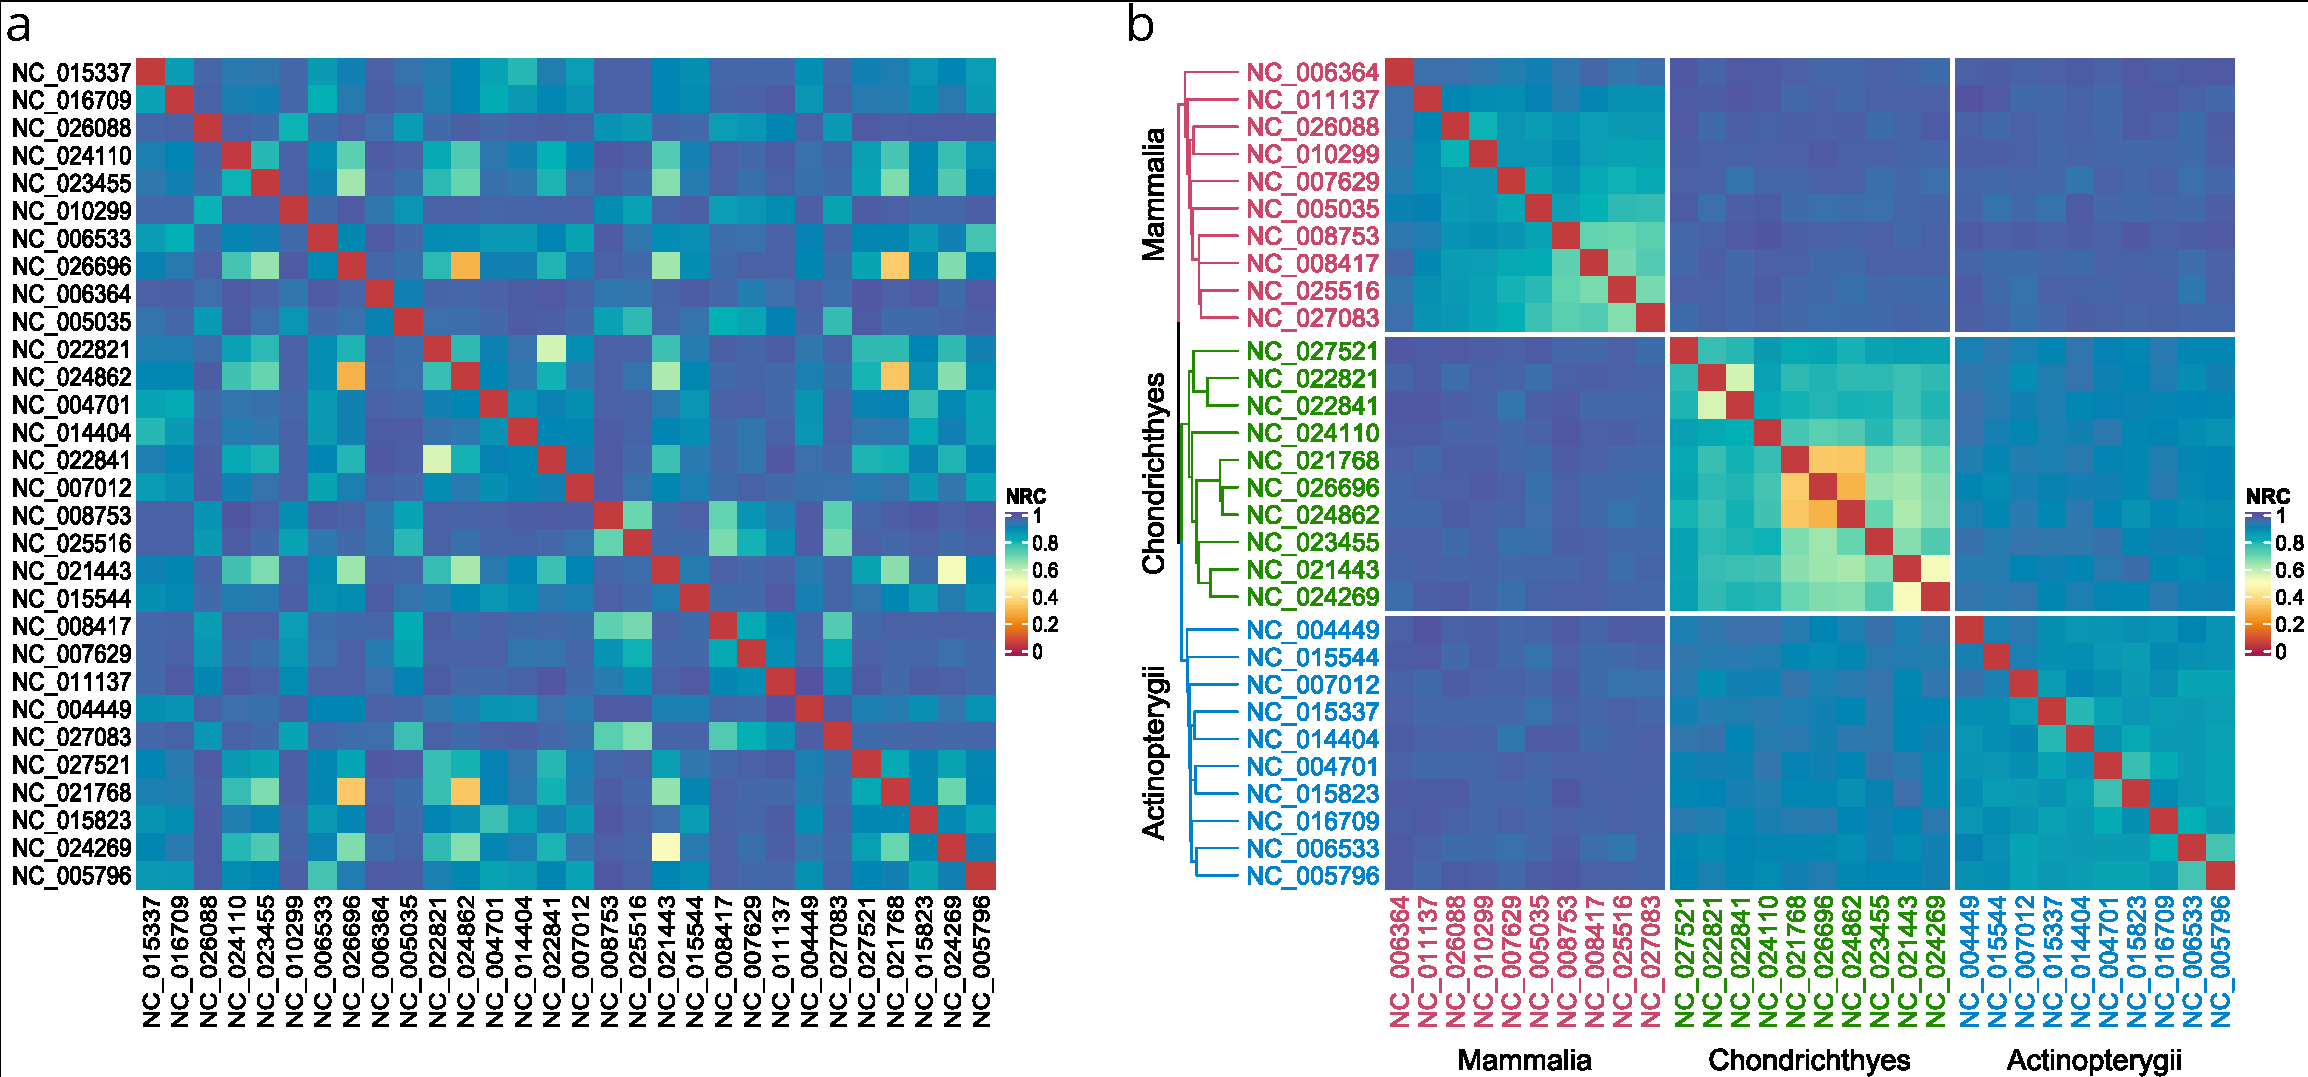
\includegraphics[width=\textwidth]{fig.pdf}
   \caption{NRC.}
   \label{fig.nrc}
\end{figure*}


\bibliography{ref}
\end{document}